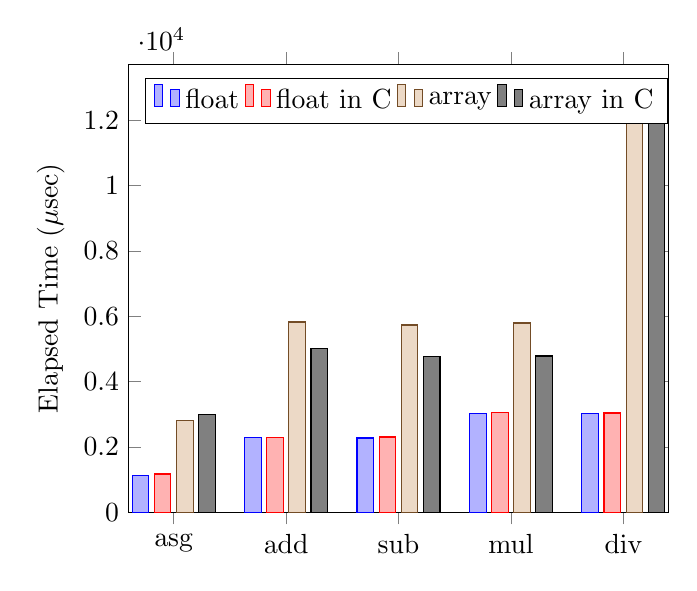
\begin{tikzpicture}
\begin{axis}[
  ybar, bar width=6pt,
  ylabel=Elapsed Time ($\mu$sec),
  symbolic x coords={asg, add, sub, mul, div},
  legend pos=north west, legend columns=4]
\addplot coordinates
  {(asg, 1134.2) (add, 2277.2) (sub, 2271.8) (mul, 3034) (div, 3029.2)};
\addplot coordinates
  {(asg, 1168.6) (add, 2280.8) (sub, 2302.8) (mul, 3044) (div, 3039.2)};
\addplot coordinates
  {(asg, 2800.4) (add, 5823.2) (sub, 5733) (mul, 5792.2) (div, 12575)};
\addplot coordinates
  {(asg, 3000.4) (add, 5008.8) (sub, 4763.2) (mul, 4783.8) (div, 12519.6)};
\legend{float, float in C, array, array in C}
\end{axis}
\end{tikzpicture}
